\documentclass[12pt,a4paper]{report}
\usepackage{amssymb,amsthm,amsmath,amscd}
\usepackage{latexsym}
\usepackage{enumerate}
\usepackage[german]{babel}
\usepackage{verbatim}
\usepackage[hyphens]{url}
\usepackage{hyperref}
\usepackage[utf8]{inputenc}
\usepackage{pdfpages}
\usepackage{graphicx}
\usepackage{csquotes}
\usepackage[landscape]{geometry}
\begin{document}
\begin{titlepage}
	\begin{center}

		\vspace*{1.0cm}
		\huge
		\textsc{\bf{PS Algorithmen für verteilte Systeme}}

		\vspace*{4.0cm}
		\textsc{
			\normalsize{eingereicht von} \\[0.5\baselineskip]
			{\large Baumgartner Dominik, Dafir Samy}
		}

		\vspace*{3.0cm}
		\textsc{
			\normalsize{Gruppe  1(16:00)}
		}

	\end{center}
\end{titlepage}

\section*{Aufgabe 13}
Im Folgenden sind die Verteilungen der Runden- und Nachrichtenanzahlen bei Verwendung des Push, sowie des Push\&Pull Algorithmus auf einem Zufallsgraphen G(10000, 0.002) dargestellt.
Die x-Werte sind jeweils als Bereiche zu interpretieren. So beinhaltet der erste Balken im ersten Graphen beispielsweise alle Läufe, die zwischen 25 (inkliusive) und 27 (exklusive) Runden benötigten.\\
Anmerkung zur Push\&Pull Auswertung: Es wurden Werte für verschiedene c Werte aufgenommen (1,2,5,20), die angeben, wie lange die Startphase dauert. Für jeden dieser c Werte erfolgte eine Auswertung der Runden und Nachrichtenanzahlen. Am Ende wurden alle in einem x,y Diagramm vereint. Diese letzten beiden Diagramme sind nur als Überblick vorgesehen, da sich die Kategoriegrenzen bei der Vereinigung der verschiedenen Daten voneinander unterscheiden. Die Darstellung ermöglicht jedoch einen Vergleich der Ergebnisse für verschiedene c Werte. Die Farben in den Einzeldarstellungen decken sich mit jenen in der Gesamtsicht.
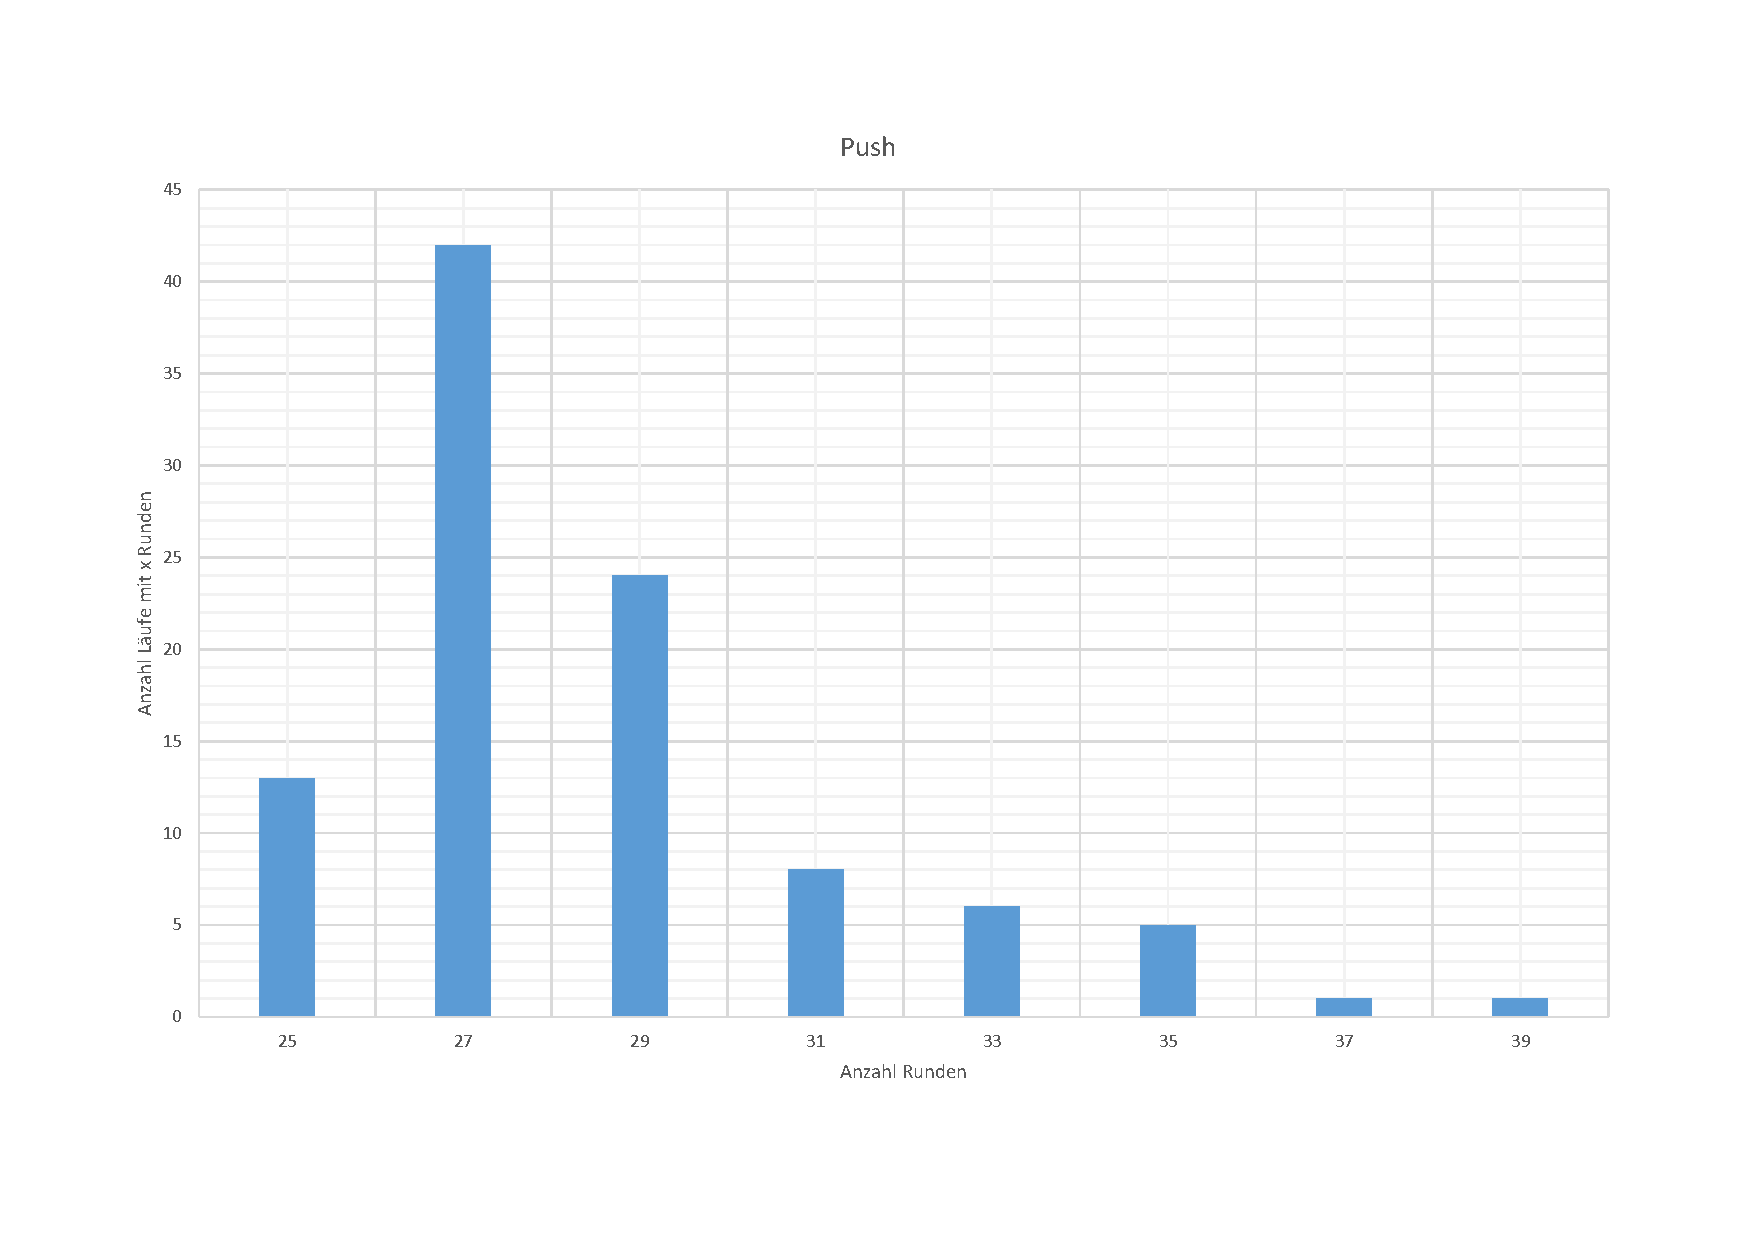
\includepdf[pages=-]{push_rnd.pdf}
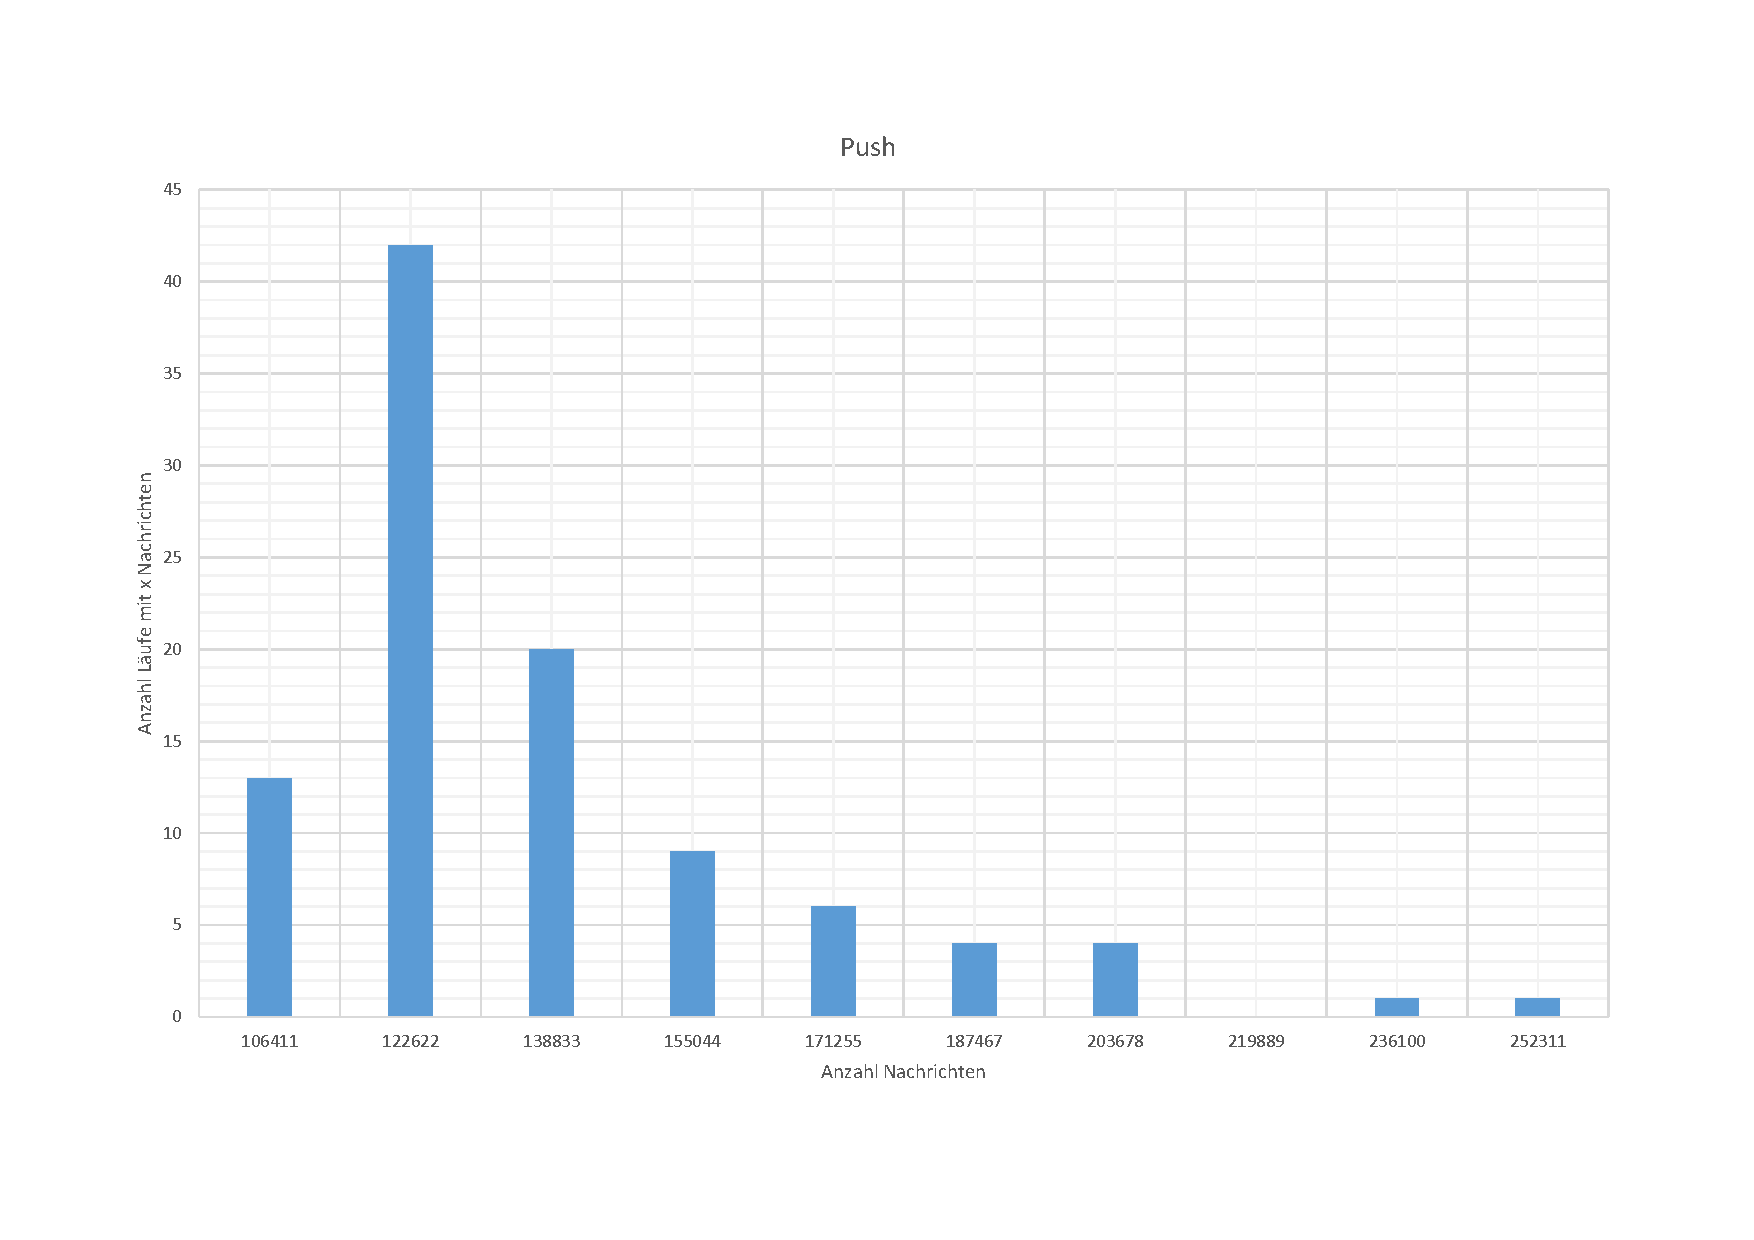
\includepdf[pages=-]{push_msg.pdf}
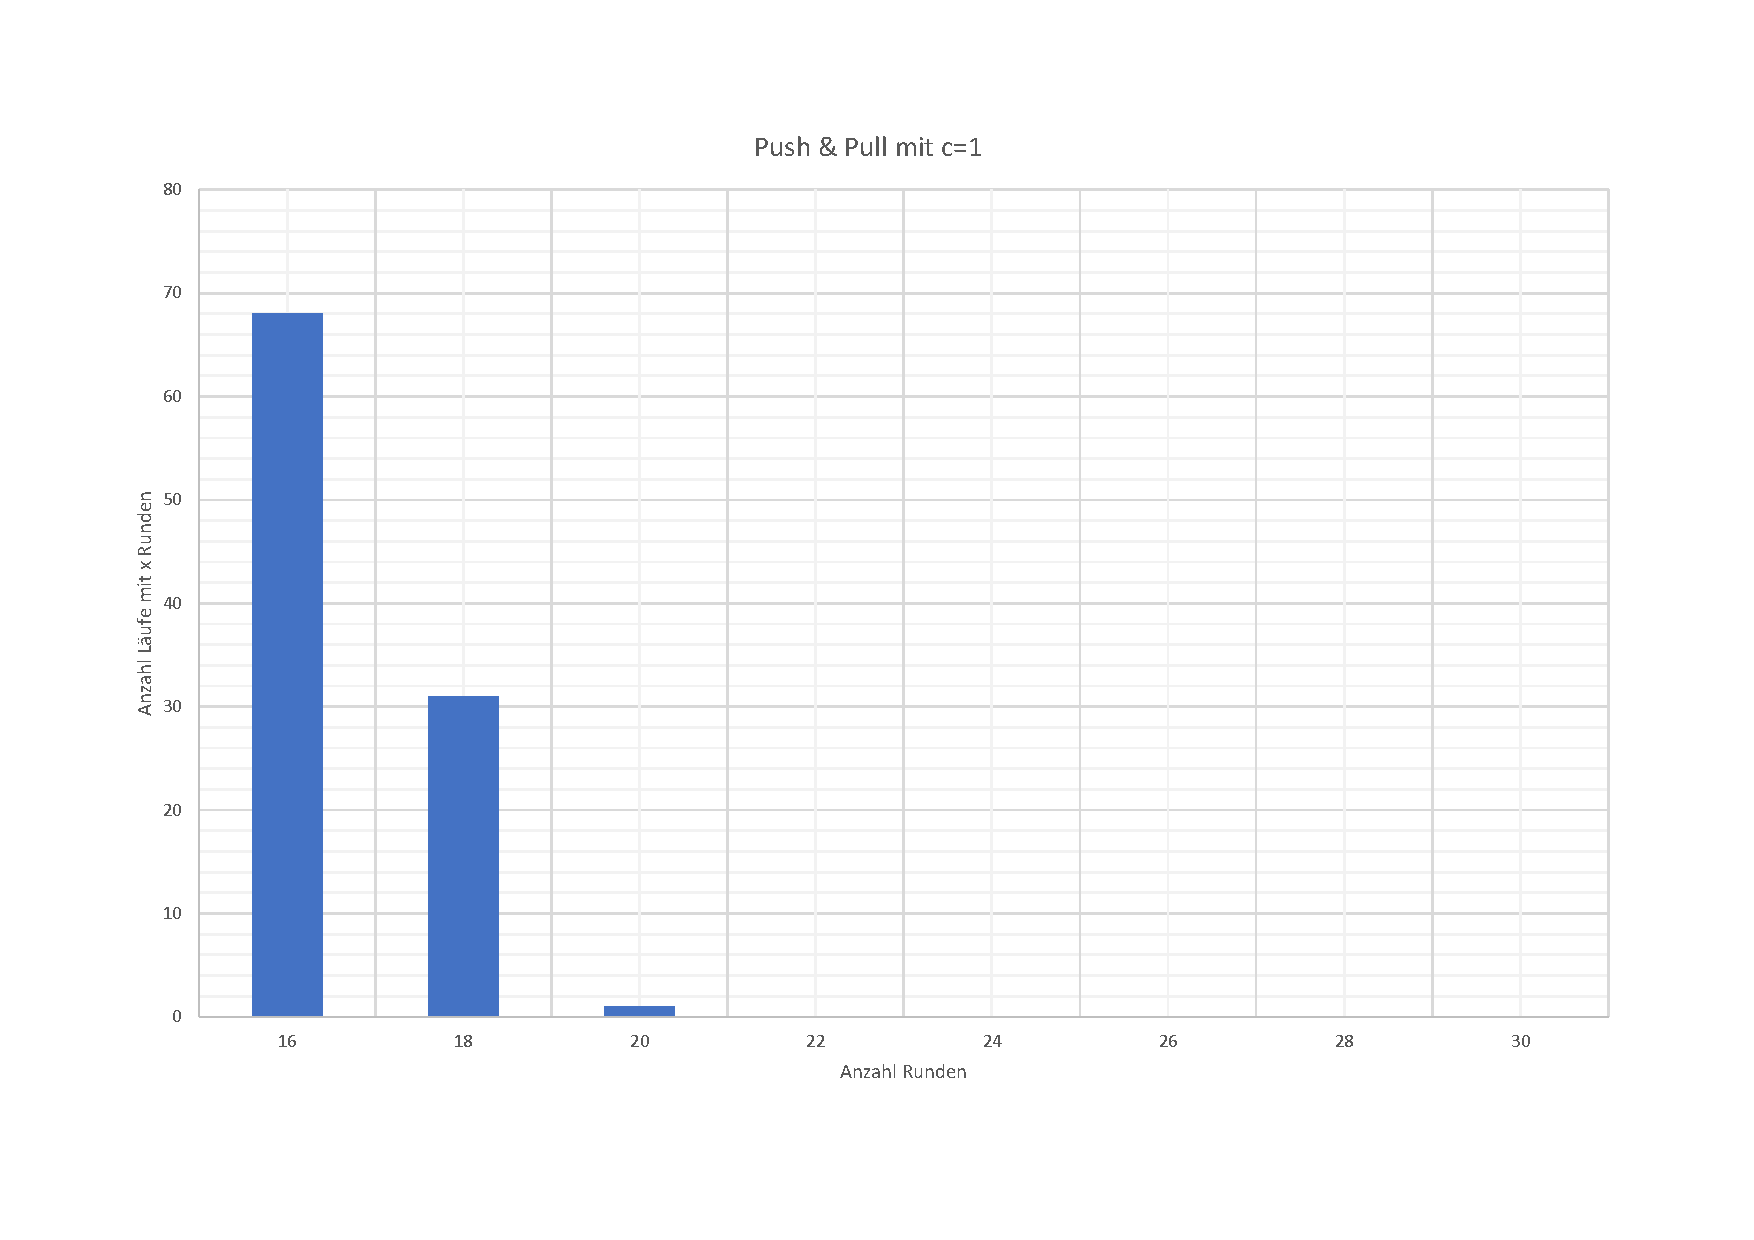
\includepdf[pages=-]{pp_r_c1.pdf}
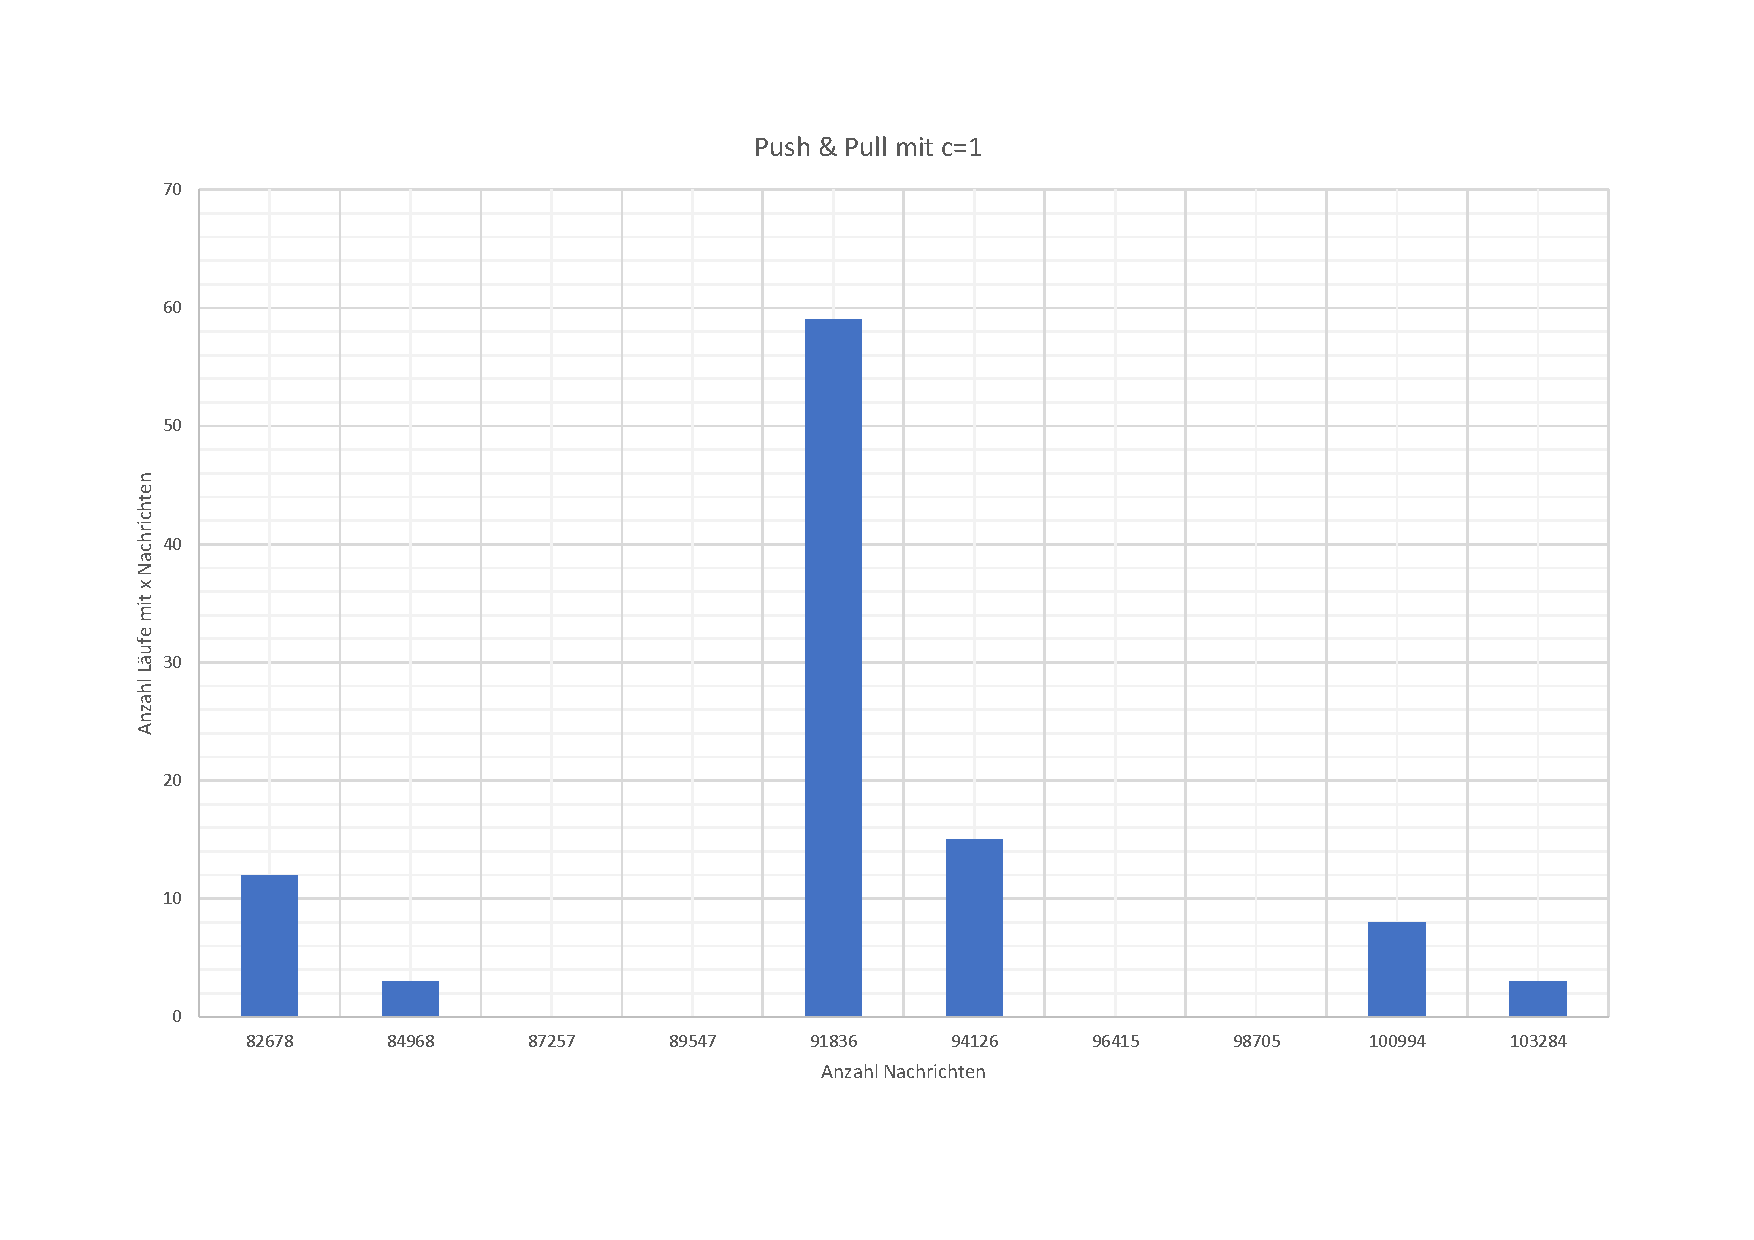
\includepdf[pages=-]{pp_m_c1.pdf}
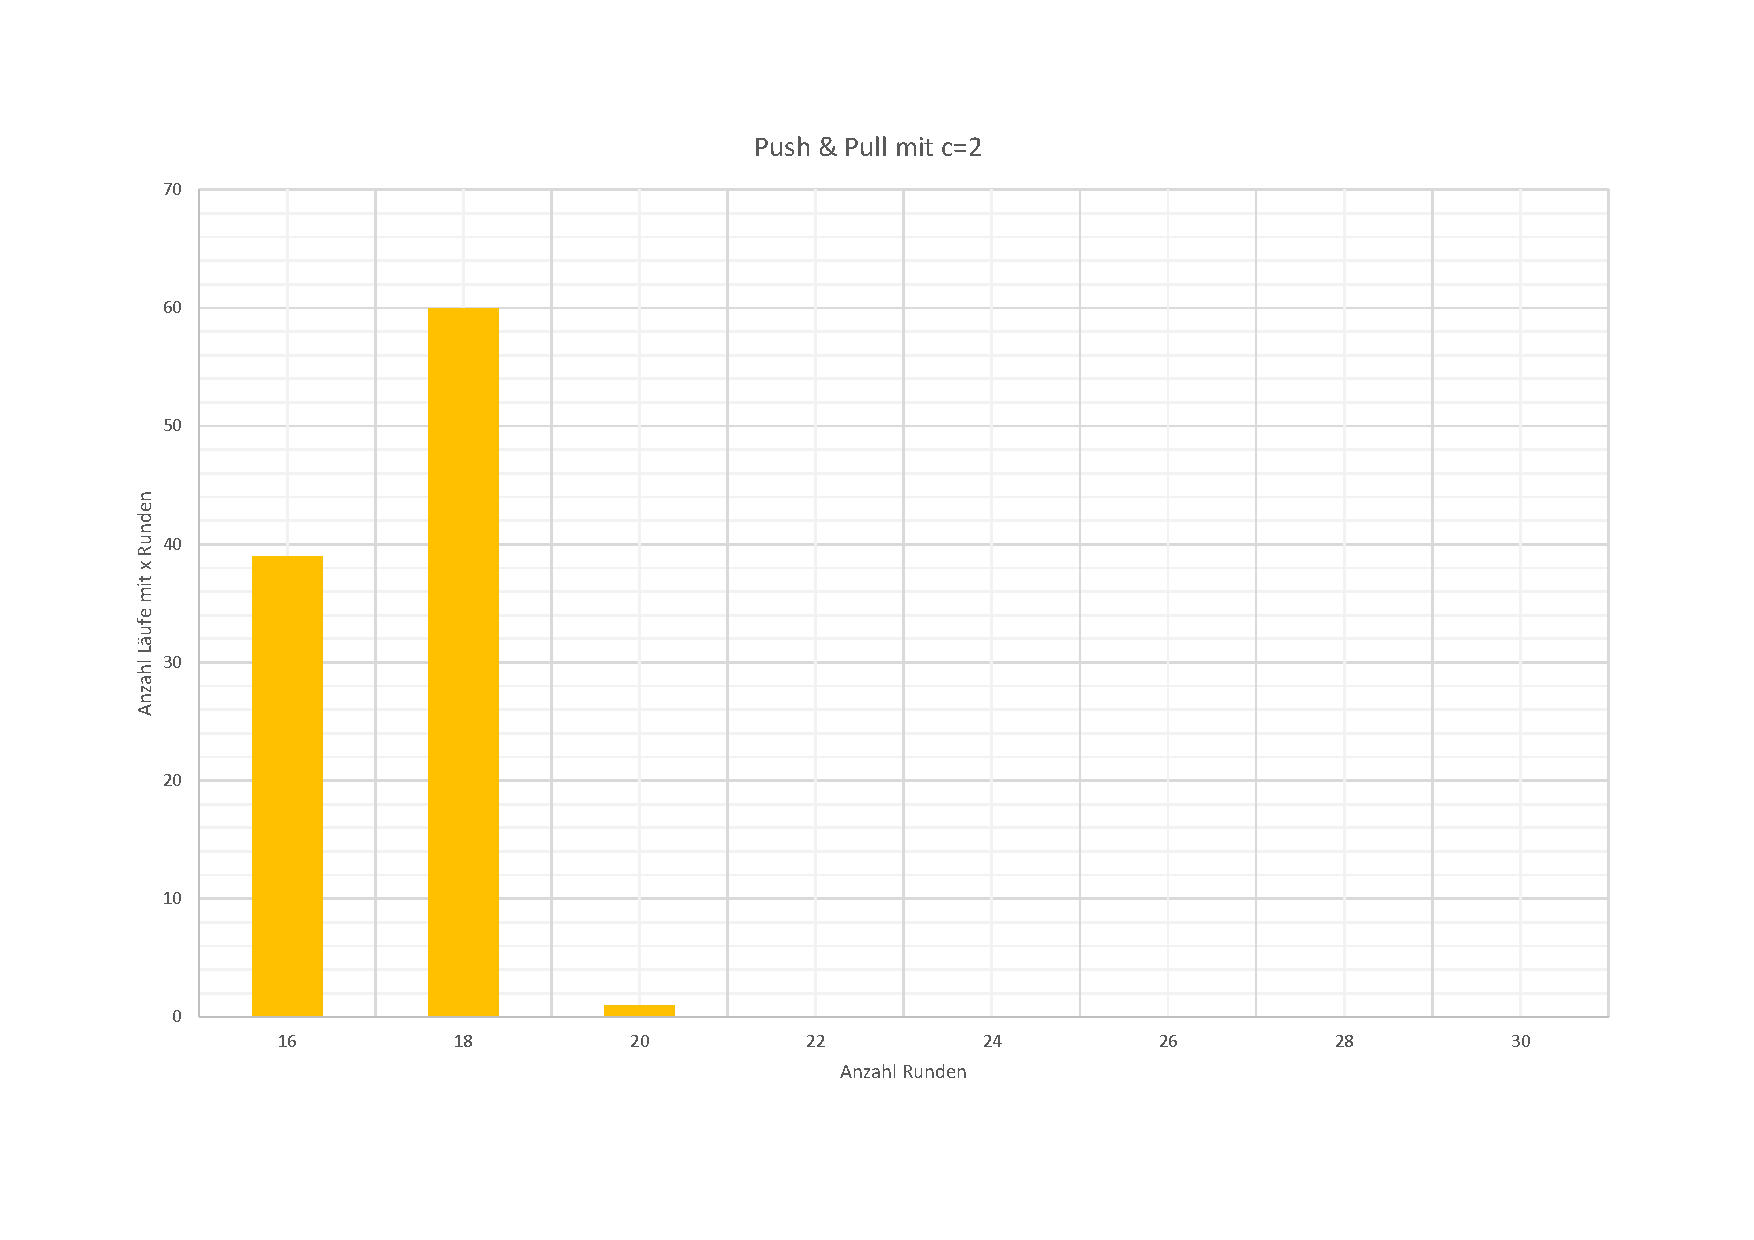
\includepdf[pages=-]{pp_r_c2.pdf}
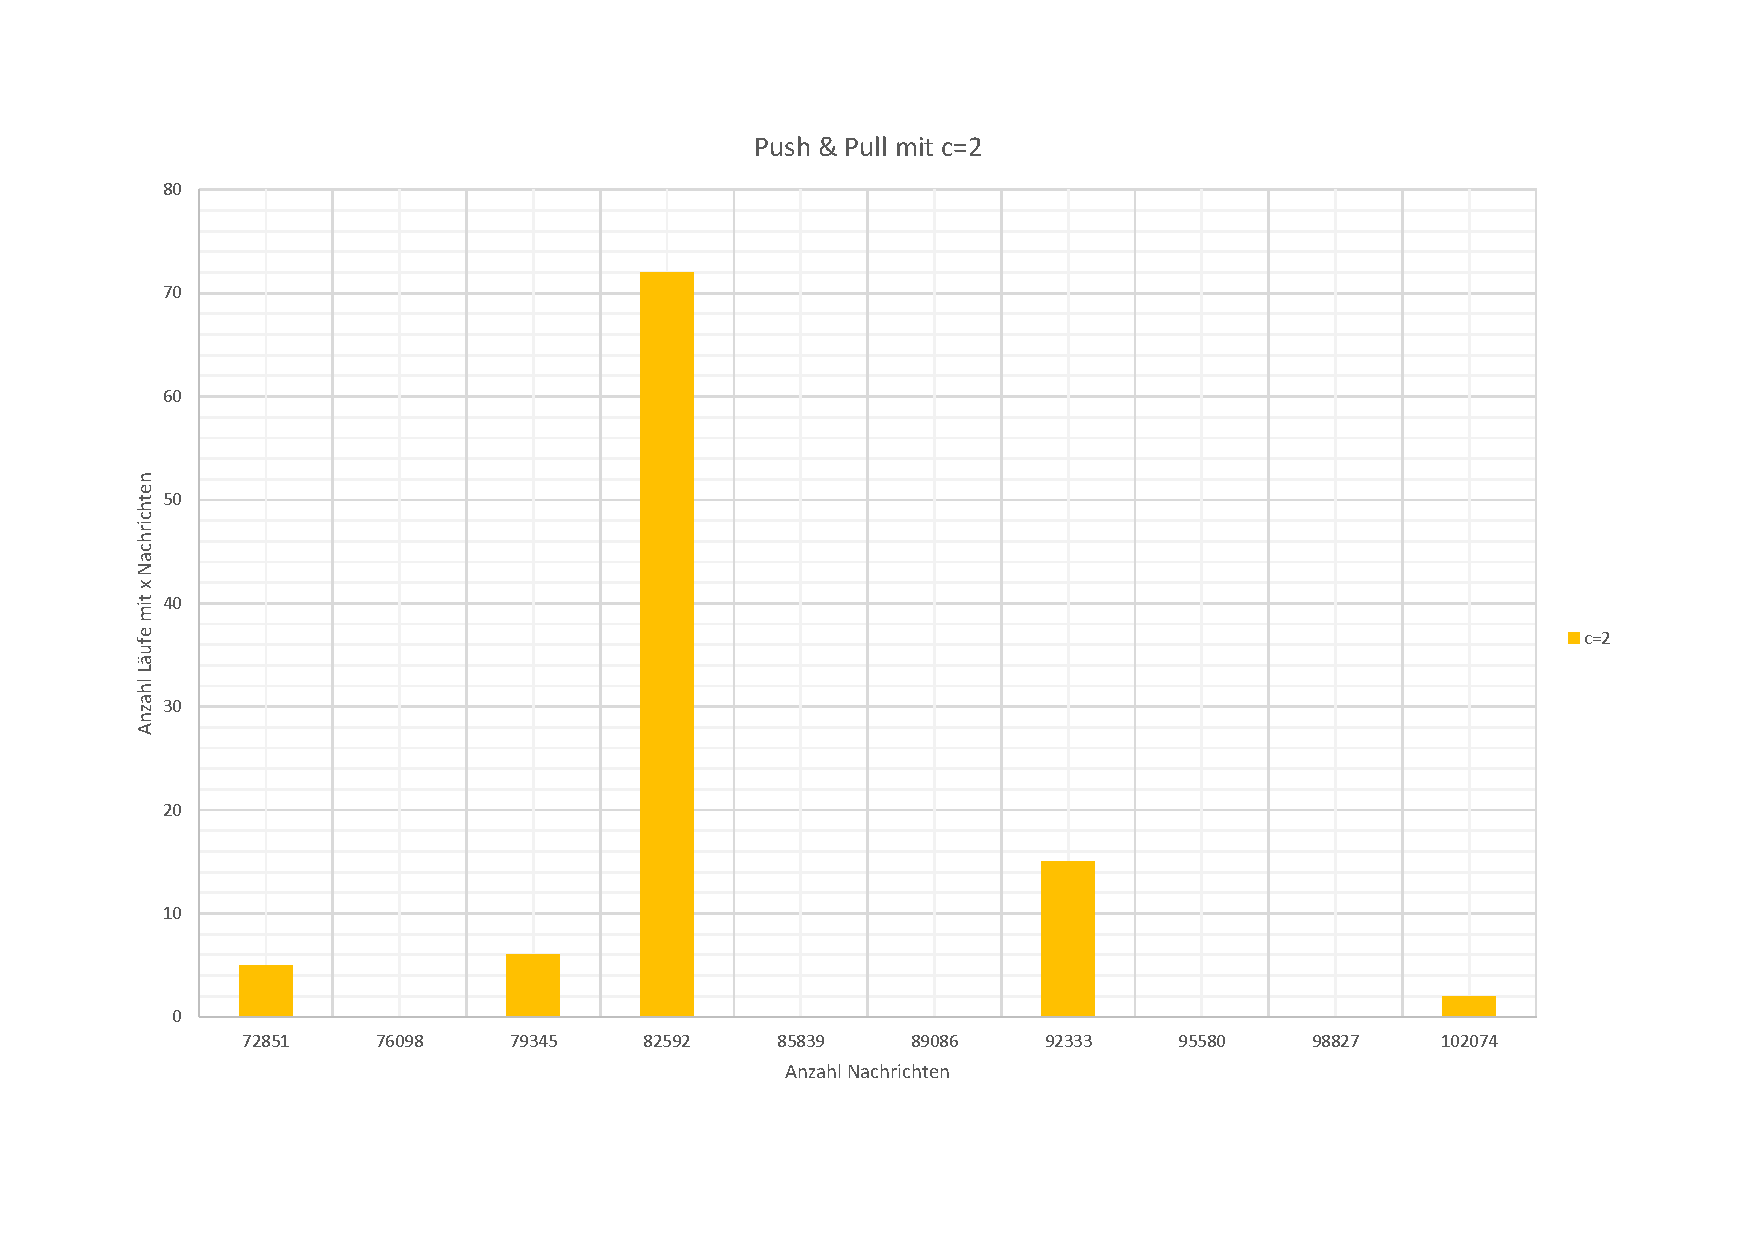
\includepdf[pages=-]{pp_m_c2.pdf}
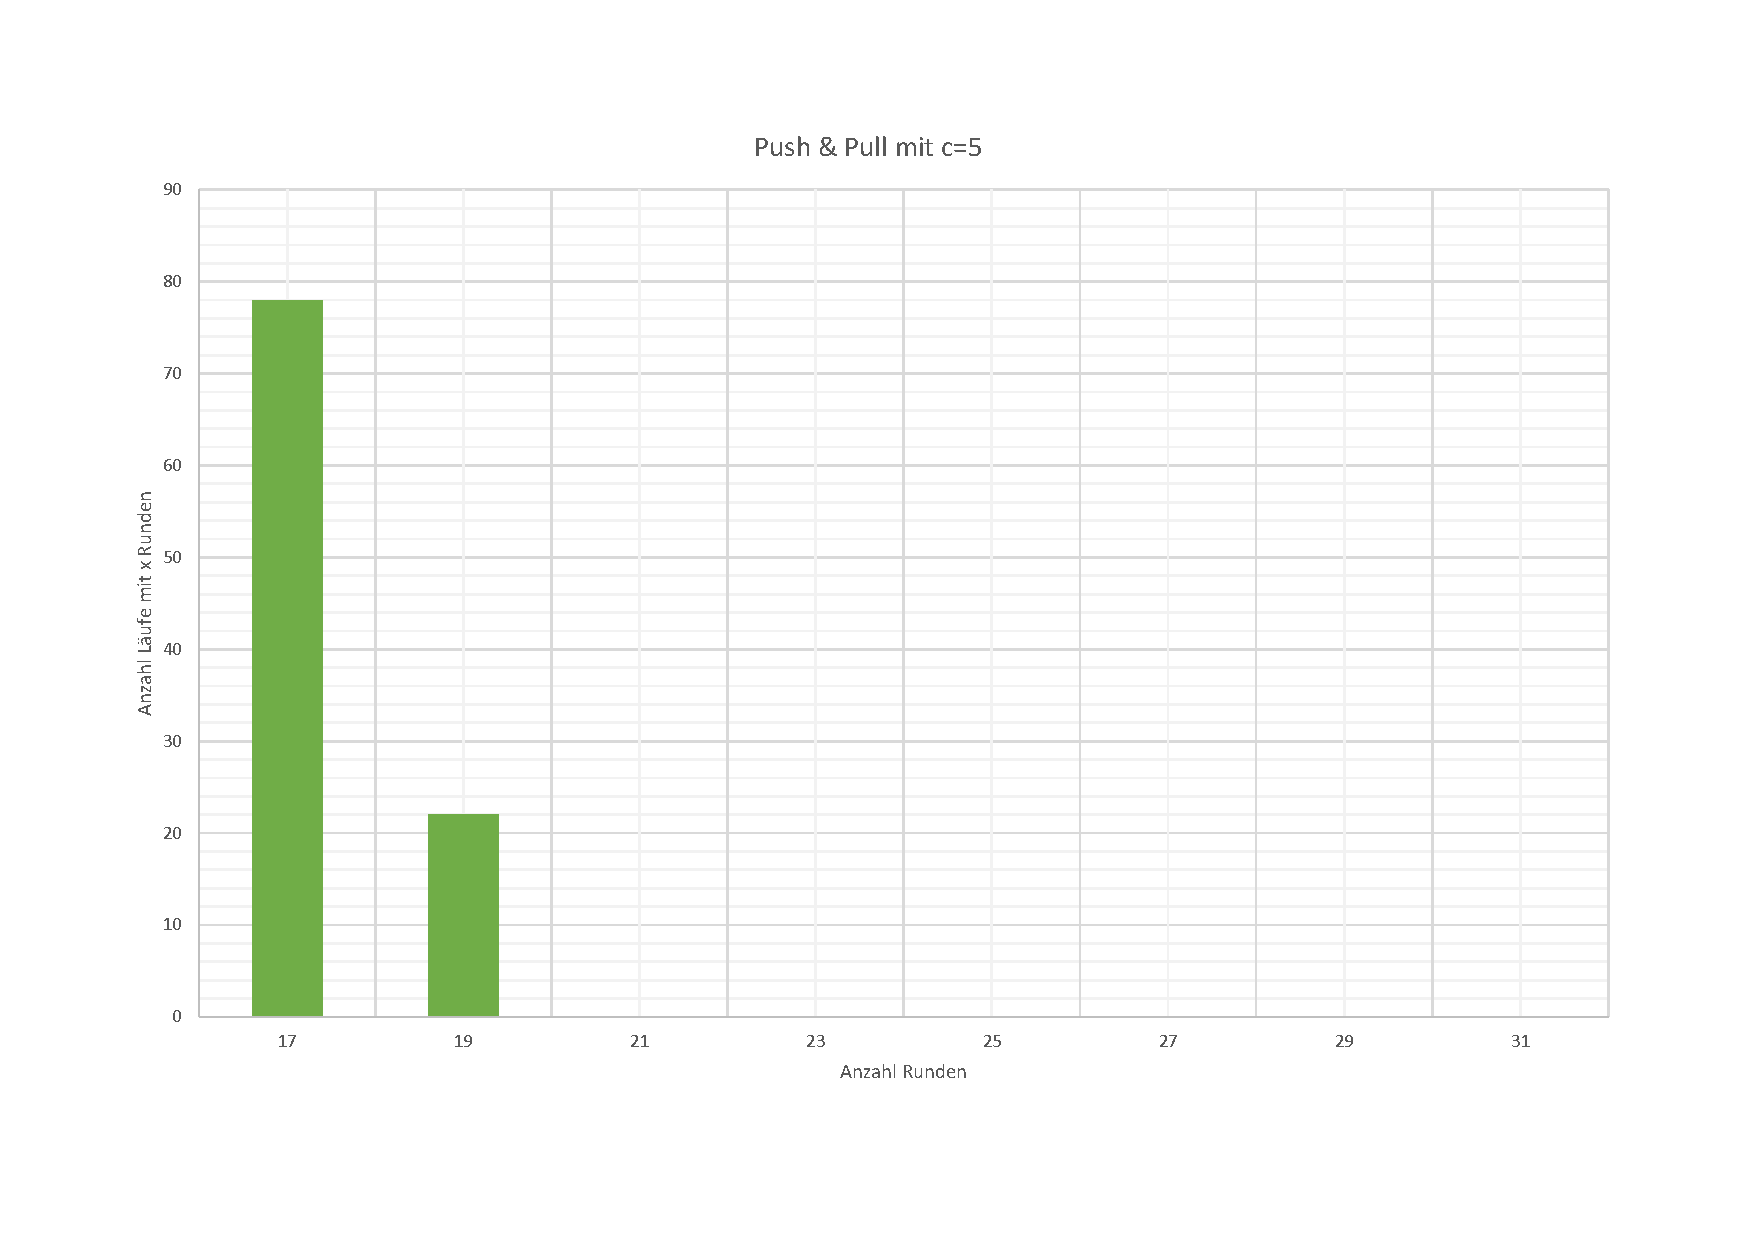
\includepdf[pages=-]{pp_r_c5.pdf}
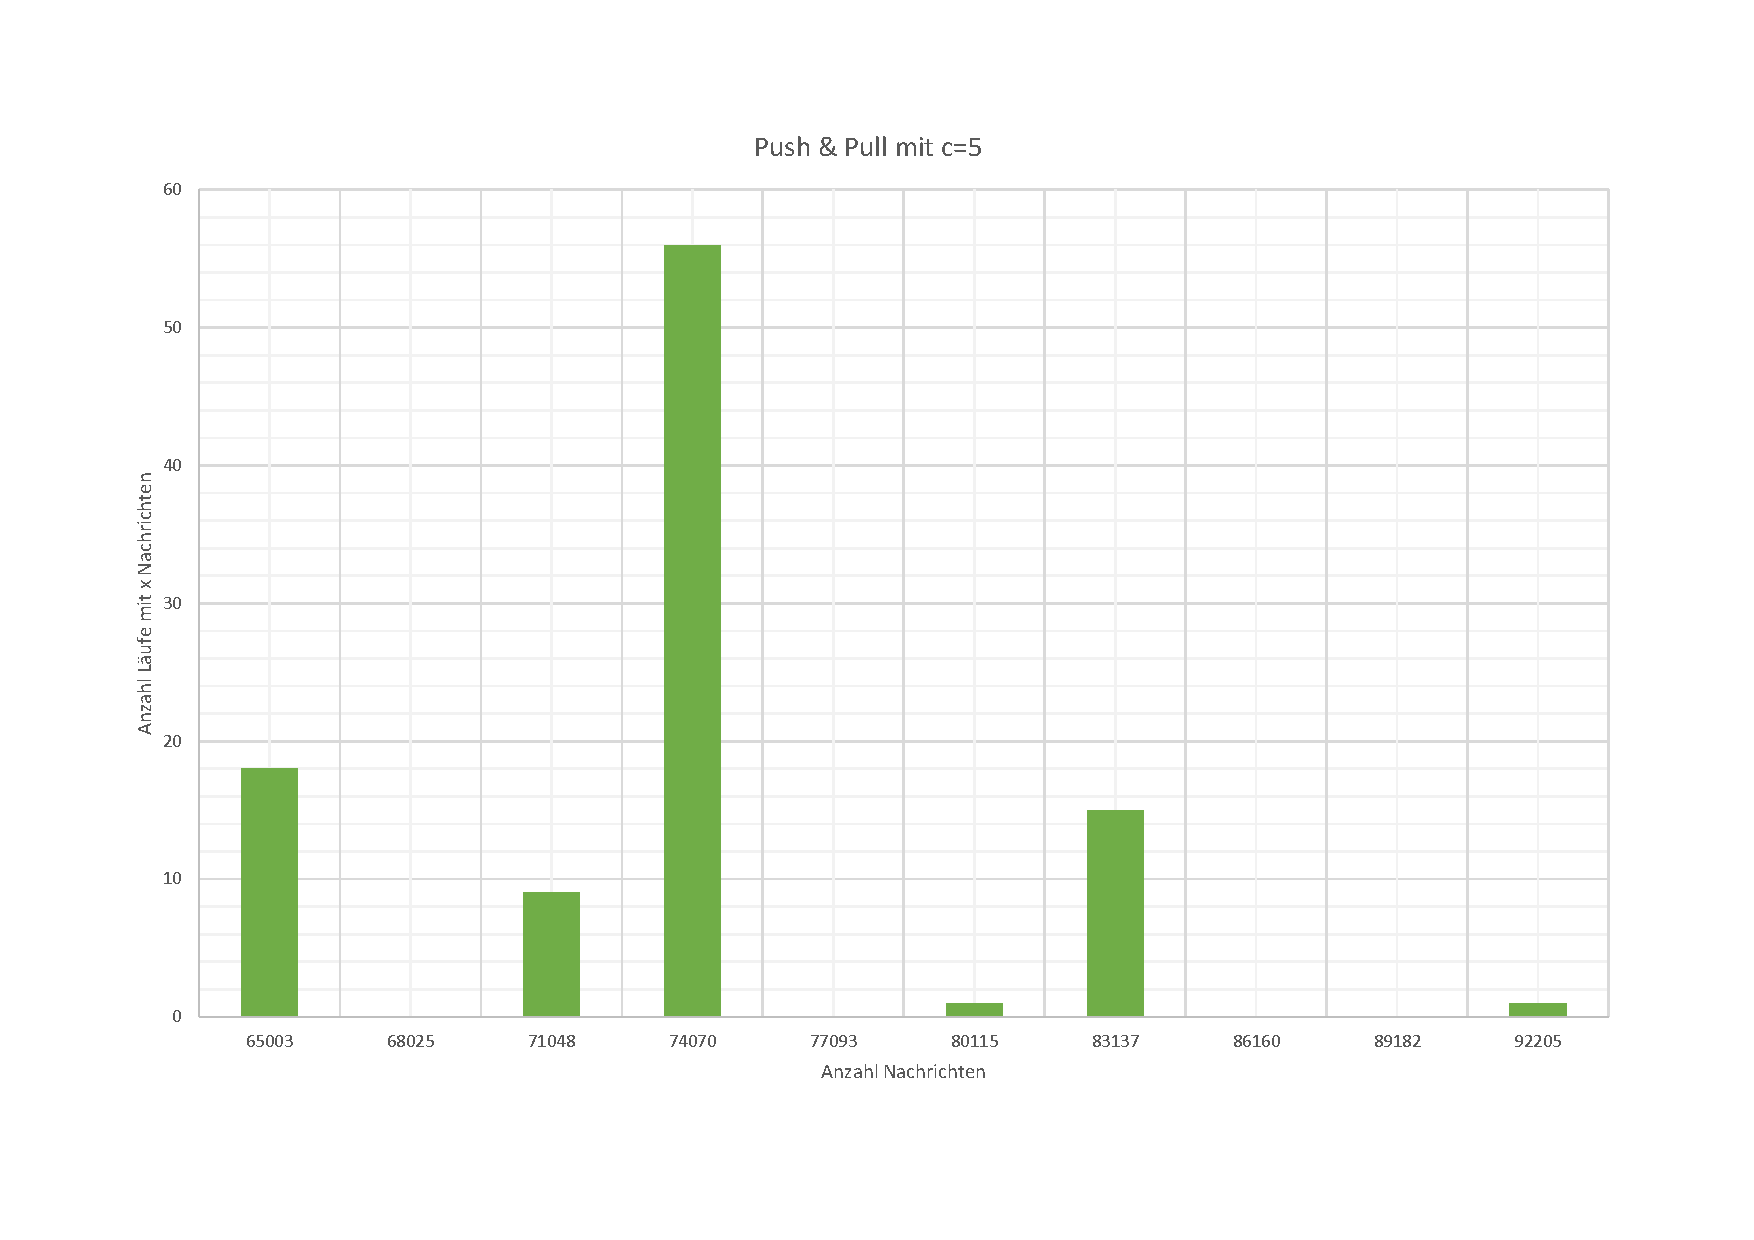
\includepdf[pages=-]{pp_m_c5.pdf}
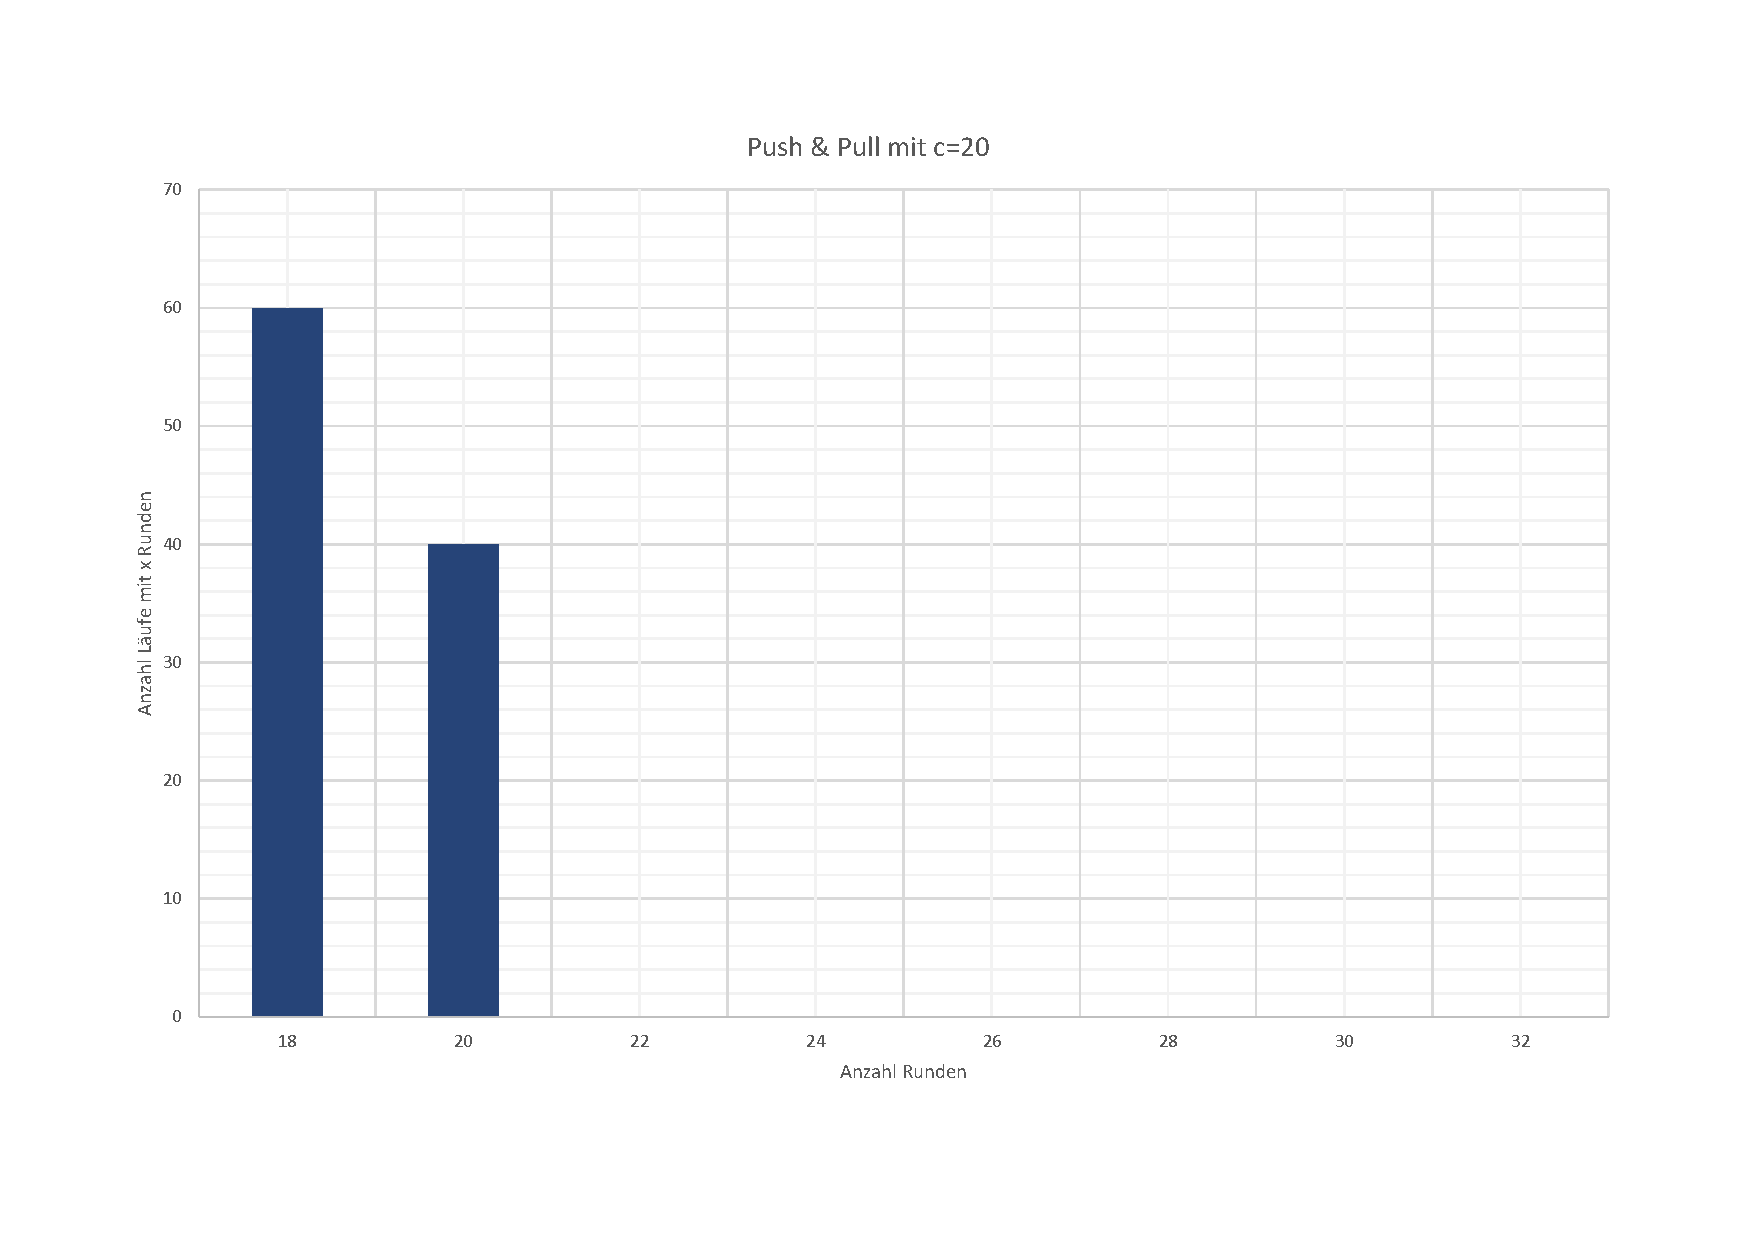
\includepdf[pages=-]{pp_r_c20.pdf}
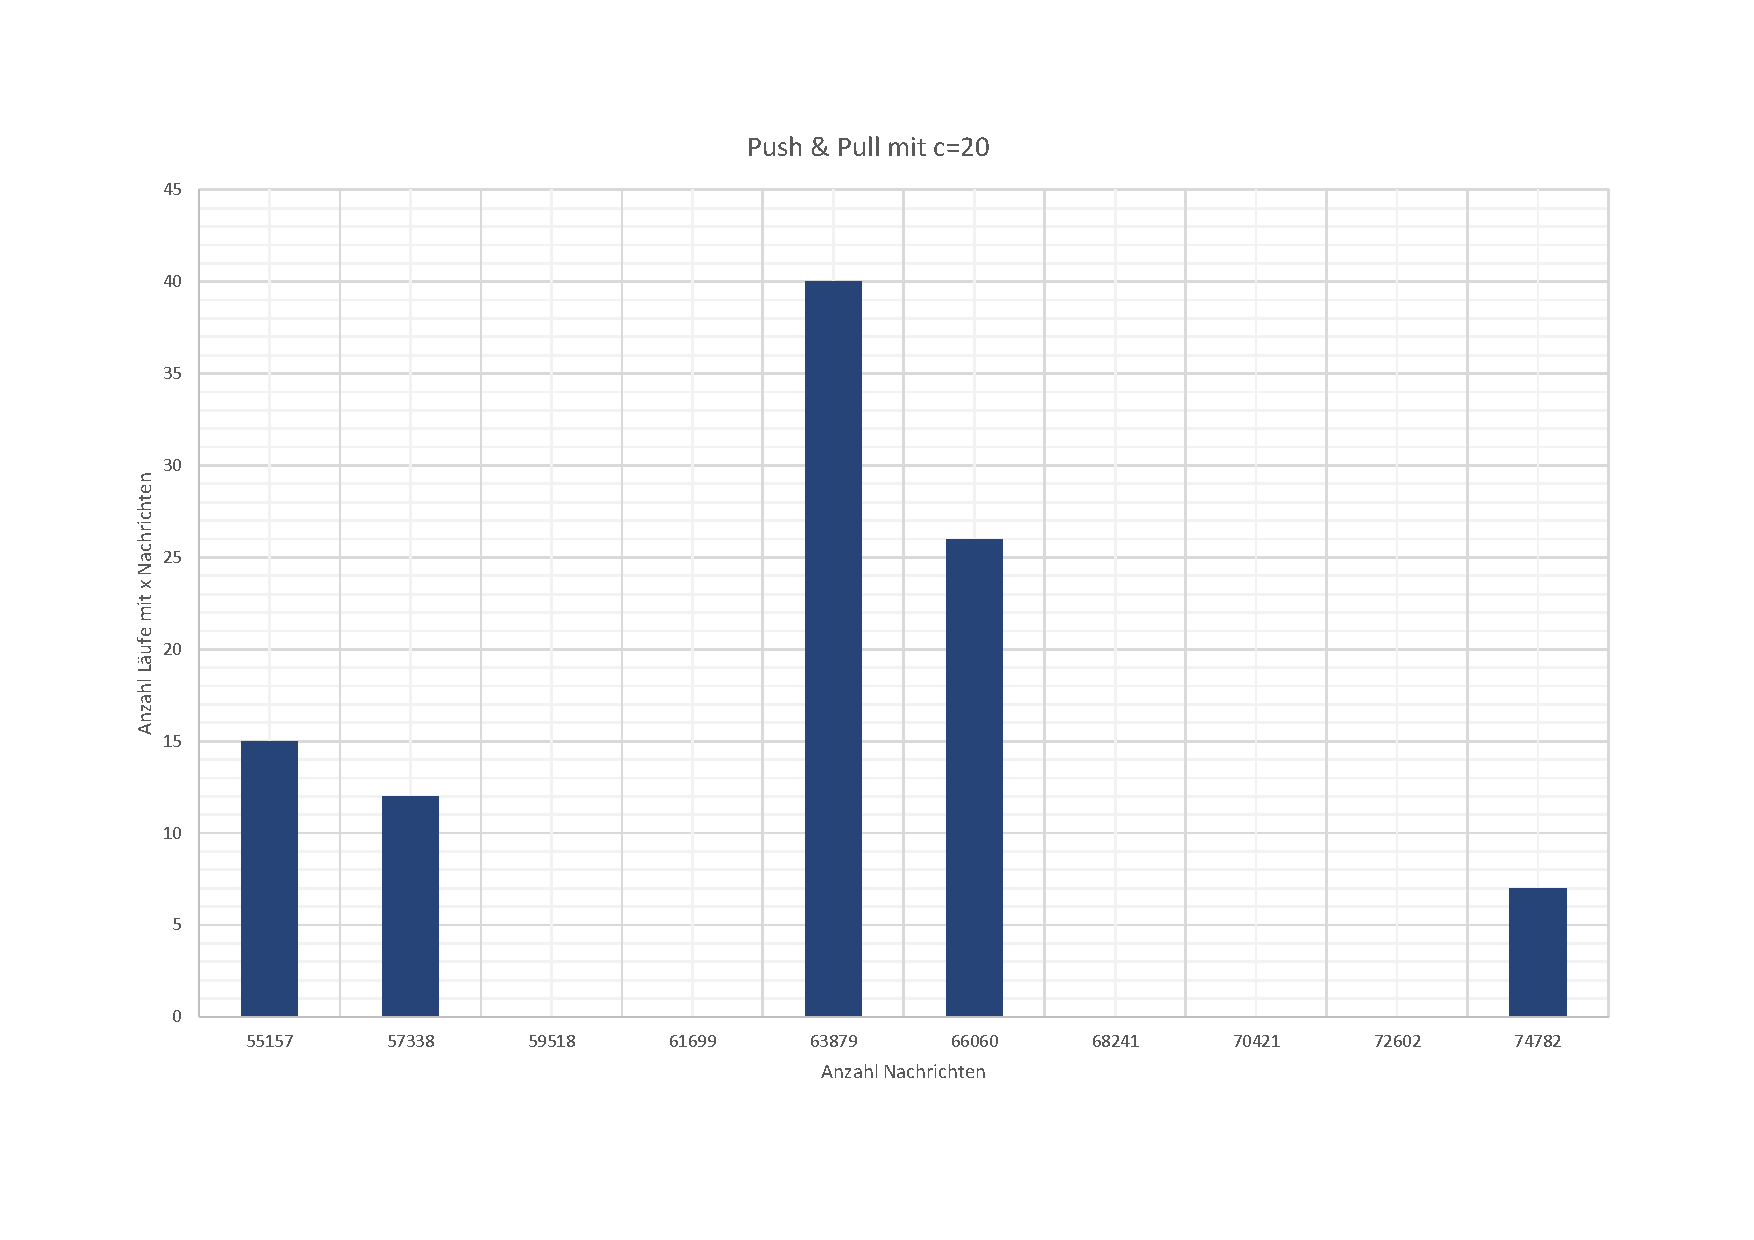
\includepdf[pages=-]{pp_m_c20.pdf}
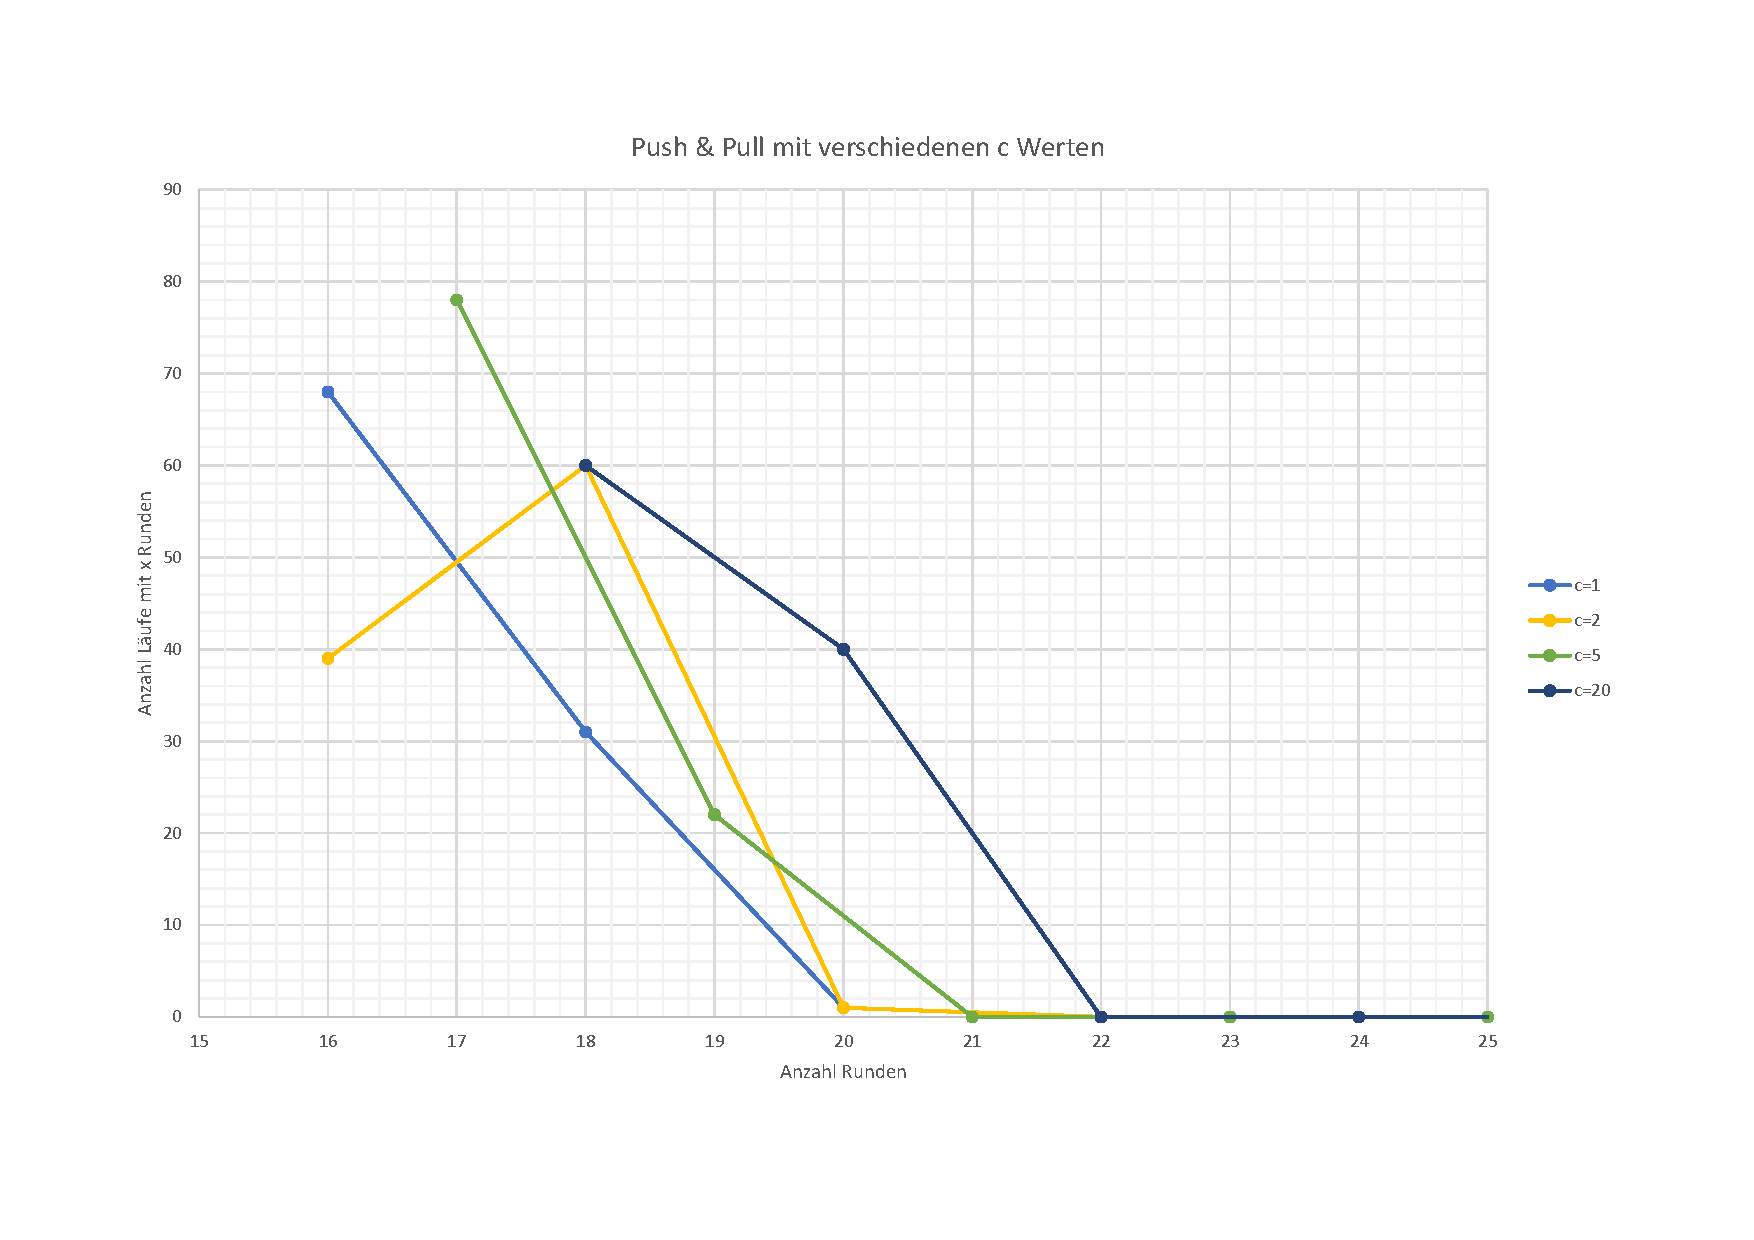
\includepdf[pages=-]{pUp_rnd.pdf}
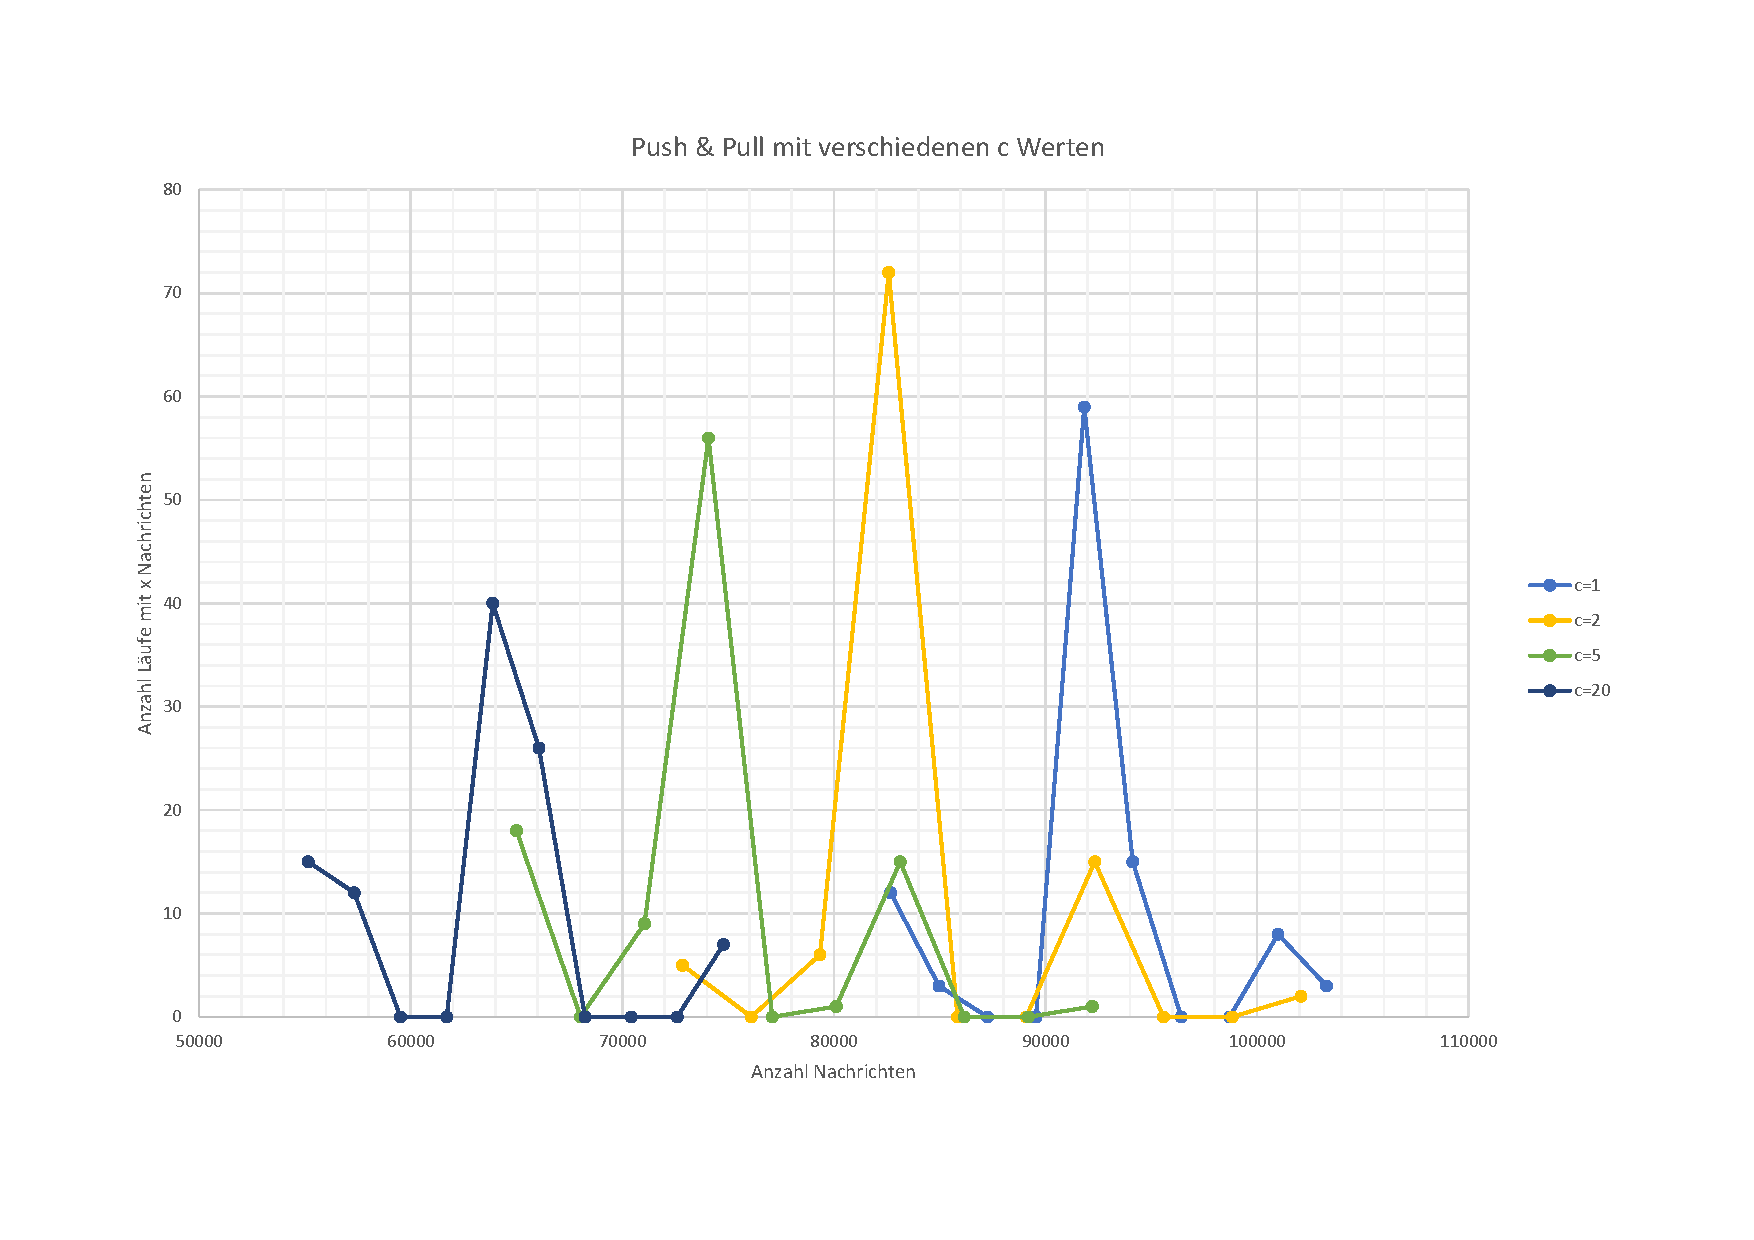
\includepdf[pages=-]{pUp_msg.pdf}
\end{document}
